\subsection{BPEL - The Overview} \label{BPEL}

In today's interconnected world, companies and businesses need to exchange data effectively and get communication flow as fast as possible, in order to save time and be more competitive. They want to automate their business processes and speed up the information exchange. BPEL is a standard that can help them to achieve this goal.
BPEL (which stands for Business Process Execution Language) is an XML standard for describing and defining business processes and hereby standardize the format of information exchange between different softwares. 

BPEL was initially developed by IBM and Microsoft. Its first version (1.0) was released in 2002 by these companies and BEA. Developers wanted to merge IBM's WSFL and Microsoft's XLANG. Both WSFL and XLANG have the same purpose - to combine web services in supporting business processes. During the following year, other companies (Siebel Systems and SAP) joined the development of BPEL and one year later they released version 1.1 together. After this, BPEL was passed to the OASIS nonprofit consortium. In 2007 Web Services BPEL (WS-BPEL) version 2.0 standard was released. During the year 2005 OASIS announced development of extension of WS-BPEL called BPEL4People, including the human interaction in BPEL processes \cite{BPELonWikipedia}.



\paragraph{BPEL Architecture example} \label{BPELarchitecture}
This paragraph contains a brief example of a simple BPEL server and its description. 
In a typical, scenario BPEL process is run on some BPEL engine which is accessible through web services (which among other things contributes to BPEL Architecture platform and operating system independence). After deploying the process, the engine waits for a request (WSDL messages) from clients (which can be for example another BPEL server or a web interface). After the request is received, the BPEL engine creates an instance of a BPEL process and runs it. When running, the process can further interact with the client and also with different BPEL servers. At the end of the operation the result is sent to the client and the process is destroyed in the server.
Note that this is not a general case since BPEL specification does not include any description of the architecture of a BPEL system and therefore this part serves for a reader to get an idea of how BPEL process works (see Figure \ref{BPELprocess}).  

\subsubsection{BPEL Activities} 
\label{BPELActivities}

In a BPEL process, activities are used to define the process logic. Activities are divided into two classes: basic and structured. 

\begin{enumerate}
\item Basic activities are those which describe elementary steps of the process behavior. The following is a list of the most important ones:
	\begin{itemize}
	\item \verb|<invoke>|
	\item \verb|<receive>|
	\item \verb|<reply>|
	\item \verb|<assign>|
	\item \verb|<throw>|
	\end{itemize}

\item Structured activities encode control-flow logic, and can contain other basic and/or structured activities recursively. The most important are listed below:
	\begin{itemize}
	\item \verb|<sequence>|
	\item \verb|<flow>|
	\item \verb|<if>|, \verb|<while>|, \verb|<repeatUntil>|  
	\item \verb|<pick>|
  \end{itemize}
\end{enumerate}


\subsubsection{BPEL Communication}
\label{BPELCommunication}
BPEL processes need to communicate with each other and for this purpose they usually use the combination of a description language, WSDL (see section \ref{Wsdl}), and a protocol, SOAP. WSDL stands for Web Services Description Language and is used to define the interfaces between communicating processes. It means that WSDL determines the format of messages, their data types and types of ports used for transmitting messages \footnote{each port has a particular type(s) assigned and therefore it can receive/send messages of this type(s) only} Whereas WSDL defines the interface between processes, SOAP works on lower level and is used for transmitting the data.

\begin{figure}
\begin{center}
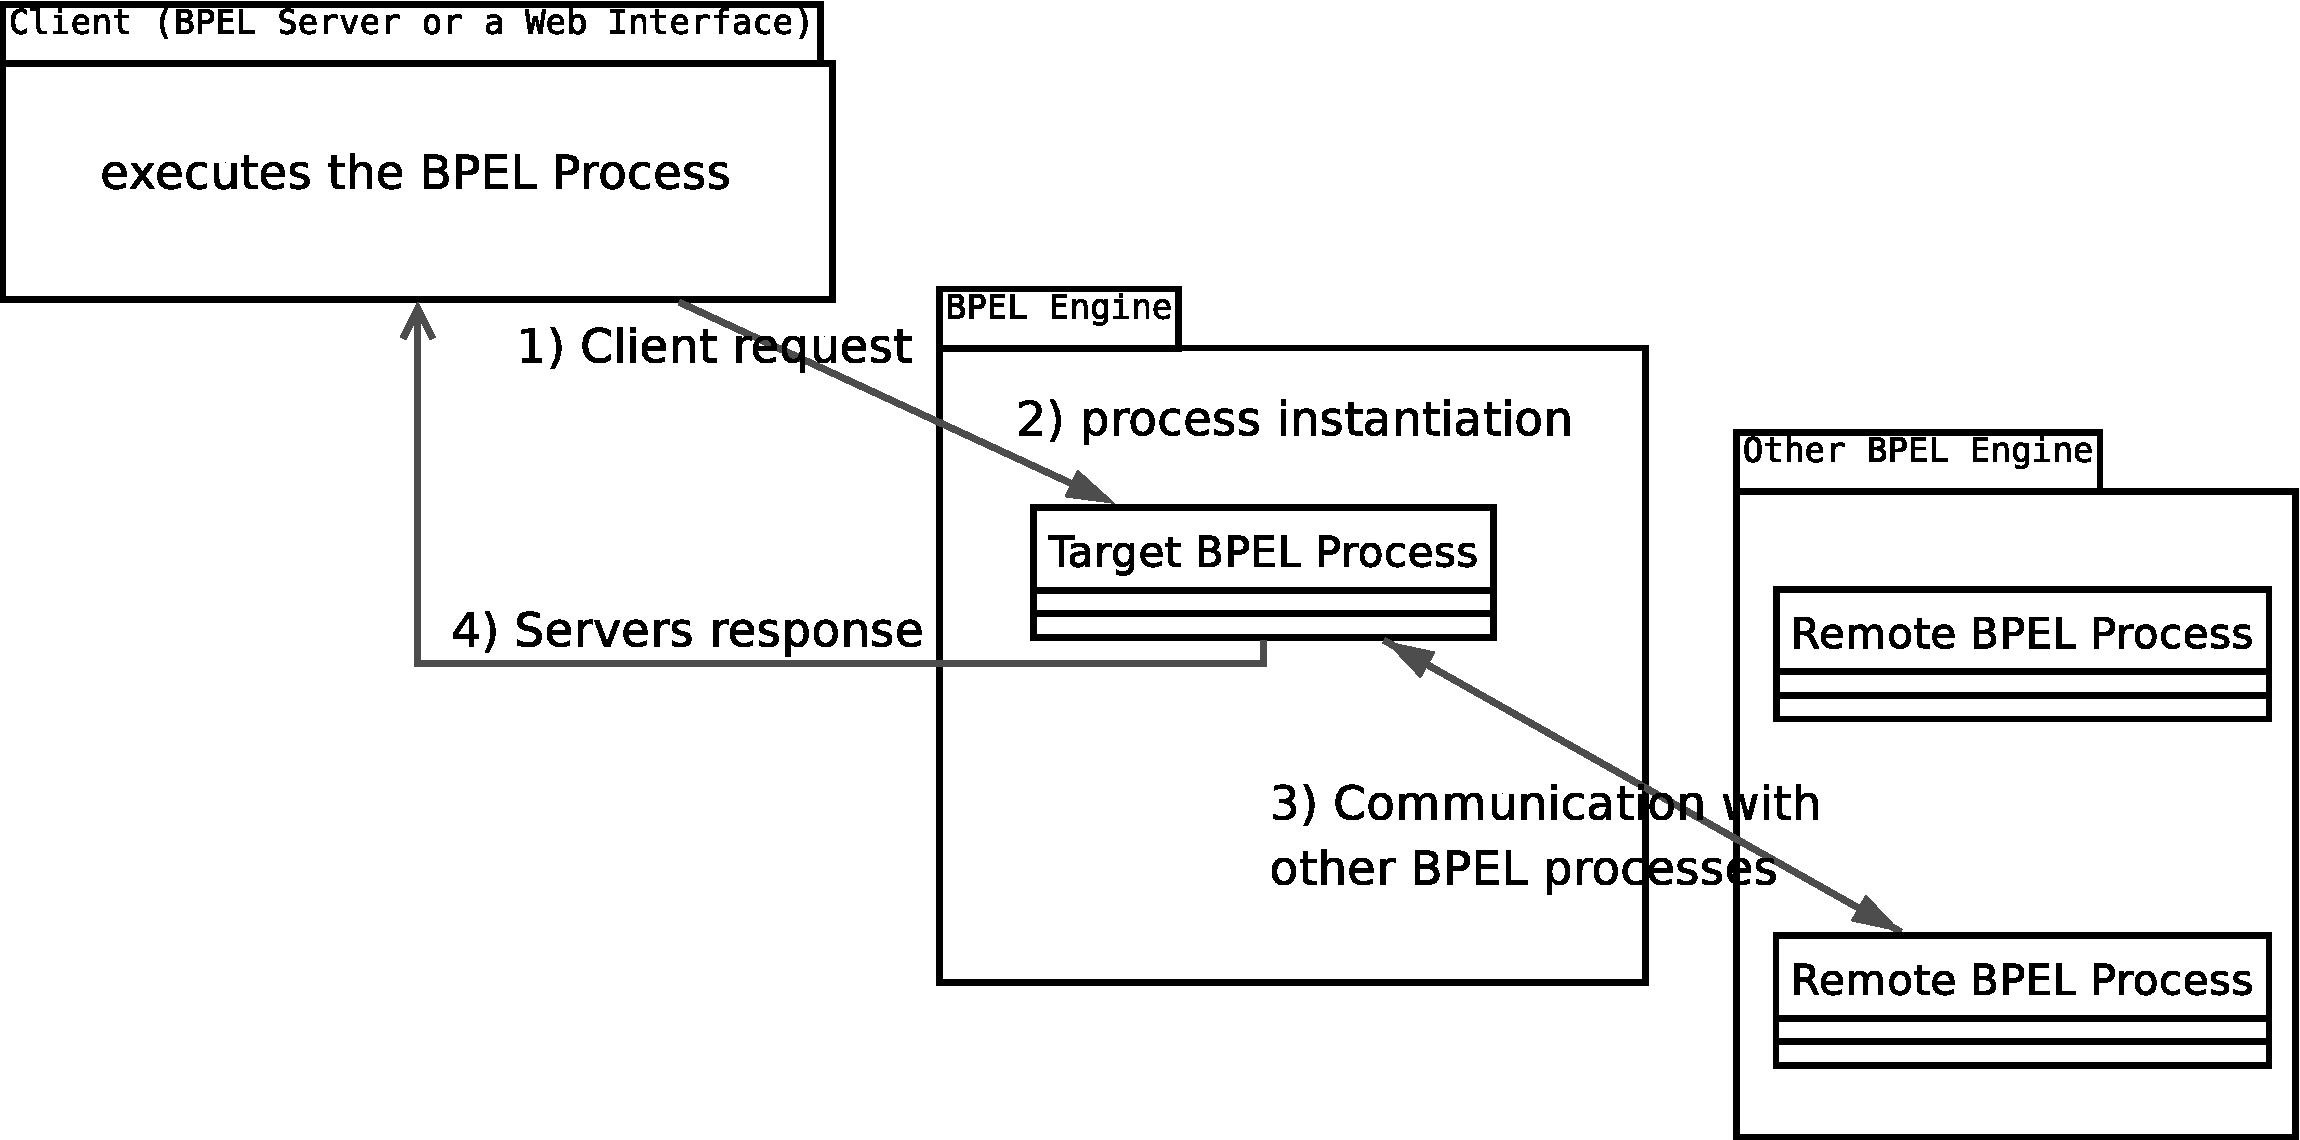
\includegraphics[width=125mm]{pictures/image-BPEL.pdf}
\caption{Execution of a simple BPEL Process}
\label{BPELprocess}
\end{center}
\end{figure}

\subsubsection{Technologies and protocols used by BPEL}
As mentioned before, BPEL uses WSDL to define process interface and SOAP for message transmitting. On lower levels XML Schema is used for defining the type of XML documents which are sent and received. On the lowest level XML is used for data encapsulation. This can also vary from implementation to implementation. For example, some engines (i.e. Oracle BPEL Process Manager) allow communication with each other using Java RMI instead of SOAP. WS-BPEL 2.0 standard also adds in the specification some new technologies like XPath for accessing data in complex variables and XSLT operations for transforming them \cite{OraBPELRMIInvocation}.


\label{BPELfiles}
BPEL is based on the XML language. As a programming language it has three basic components: the programming logic, the data types and the input/output (I/O). They are divided into three files written in three languages: BPEL, XML Schema definition and WSDL. 
The BPEL file contains the "orchestration" of the system. It specifies an executable process that involves message exchanges between the various processes composing the system. The XML Schema file is used to define the types used in the program. The WSDL file defines the Web Service from an "abstract" point of view describing all the operations for each process participating in the business service.
Table \ref{BPELfilesTable} summarizes the functionalities of the three files composing a BPEL process.

%%%%%%%    Table %%%%%%%%%%%%%%%%%%%%%%%%%%%%%%%%%%%%%%%%%%%%%%
\begin{table}[h!]
\caption{BPEL files' functionalities}
\label{BPELfilesTable}
\begin{center}
\begin{tabular}{l l l}
						\toprule
						\addlinespace[0.2cm]
\textbf{Basic Components} 	& \textbf{Language} 	& \textbf{File extension} 	\\ 
						\cmidrule(l){1-3}
Programming Logic 		& BPEL			& .bpel 			\\[0,1cm]
Data Types 			& XSD (XML Schema) 	& .xsd 				\\[0,1cm]
Input/Output 			& WSDL 			& .wsdl 			\\[0,1cm]
						\addlinespace[0.2cm]
						\bottomrule
\end{tabular}
\end{center}
\end{table}
%%%%%%%%%%%%%%%%%%%%%%%%%%%%%%%%%%%%%%%%%%%%%%%%%%%%%%%%%%%%%%


\paragraph{BPEL Engines}
Table \ref{BPELengines} represents several common BPEL engines developed by various companies \cite{BPELenginesComparisonOnWikipedia}. In this document we do not go deep into the engines' details as we concentrate more on the BPEL process, its orchestration and its functionalities. Of course, sometimes it is not possible to explain BPEL concepts without a basic knowledge about the engines. Thus, brief explanations are provided when necessary.


%%%%%%%%% Table %%%%%%%%%%%%%%%%%%%%%%%%%%%%%%%%%%%%%%%%%%%%%%%%%%%%%%%%%%%
\begin{table}
\caption{List of BPEL engines}
\label{BPELengines}
\begin{center}
\begin{tabular}{l l l}  %\begin{tabular}{|p{5.5cm}|p{3cm}|p{2.5cm}|}
						\toprule
						\addlinespace[0.2cm]
{\bf Name of BPEL Engine} 	& {\bf Supported BPEL Version} 	& {\bf License} 	\\
						\cmidrule(l){1-3}
ActiveBPEL         		& BPEL4WS 1.1, WS-BPEL 2.0 	& GPL and commercial 	\\[0,1cm]
Apache ODE         		& WS-BPEL 2.0 			& Apache license	\\[0,1cm]
jBMP (jBoss)         		& WS-BPEL 2.0 			& LGPL			\\[0,1cm]
Open ESB (Oracle)		& WS-BPEL 2.0 			& Open Source		\\[0,1cm] 
Oracle BPEL Process Manager   	& BPEL4WS 2.0 			& commercial		\\[0,1cm]
WebSphere Process Server (IBM)	& WS-BPEL 2.0			& commercial		\\[0,1cm]
						\addlinespace[0.2cm]
						\bottomrule
\end{tabular}
\end{center}
\end{table}
%%%%%%%%%%%%%%%%%%%%%%%%%%%%%%%%%%%%%%%%%%%%%%%%%%%%%%%%%%%%%%%%%%%%%%%%%%%
